\documentclass[a4paper, 12pt]{article}
\usepackage[utf8]{inputenc}
\usepackage[portuguese]{babel}
\usepackage{mathptmx}
\usepackage{enumitem}
\usepackage{amsmath}

% Margins
\usepackage{geometry}
\geometry{left=30mm,right=20mm,%
	bindingoffset=0mm, top=30mm,bottom=20mm,includefoot}

% Images
\usepackage{graphicx}
\graphicspath{ {./images/} }

% Title font size
\usepackage{titlesec}
\titleformat*{\section}{\bfseries}

% Indent first sentence of a paragraph
\usepackage{indentfirst}

% highlight code
\usepackage{listings}

% Page numbers at bottom right
\usepackage{fancyhdr}
\pagestyle{fancy}
\fancyhf{}
\renewcommand{\headrulewidth}{0pt}
\rfoot{\thepage}

% 1.5 line spacing (yes, 1.25 is actually 1.5)
\fontsize{10}{12}
\linespread{1.50}
\fontfamily{ptm}
\selectfont

% Fix vspacing for section titles
\let\oldsection\section
\renewcommand{\section}[1]{{\vspace{20pt}\oldsection*{#1}\vspace{-10pt}}}

% Indent size
\setlength\parindent{10mm}

% Jump 20pt
\newcommand{\jump}[1]{{\vspace{20pt}}}

\newenvironment{leftquote}[1][]
{
	\hspace{30pt} #1
	\vspace{20pt}
	\fontsize{10}{10}\selectfont
	\begin{flushright}
		\begin{minipage}{120mm}
		}
		{
		\end{minipage}
	\end{flushright}
	\par
	\vspace{20pt}
}

\newcommand{\tmp}{}

\newenvironment{container}[3]
{
	\renewcommand{\tmp}{#3} %gambiarra
	
	\begin{center}
		\begin{minipage}{#1}
			\centering
			#2
		}
		{
			\raggedright
			{\footnotesize \tmp}
		\end{minipage}
	\end{center}
}

\begin{document}
	
	% Remove page number
	\clearpage
	\thispagestyle{empty}
	
	\begin{bfseries}
		\begin{center}
			
			
\includegraphics[scale=0.45]{ufc.png} \\
			\vspace{-4pt} 
			UNIVERSIDADE FEDERAL DO CEARÁ \\
			\vspace{4pt} 
			CENTRO DE TECNOLOGIA \\
			\vspace{4pt} 
			DEPARTAMENTO DE TELEINFORMÁTICA \\
			\vspace{4pt}
			\vspace{4pt}
			SEMESTRE 2025.1 \\
			
			
			\vspace*{\fill}
			\textbf{Relatório dos Homeworks de Álgebra Multilinear}
			\vspace*{\fill}
			
		\end{center}
		
		\begin{itemize}[leftmargin=*]
			\setlength{\itemsep}{0pt}
			\item[] ALUNO: Ruan Pereira Alves
			\item[] MATRÍCULA: 569551
		\end{itemize}
		
	\end{bfseries}
	\newpage
	
	\section{Homework 00}
	
	Para o item A
	Geramos aleatoriamente A e B em uma simulação de monte carlo com 1000 etapas. Por conta do custo computacional, foi necessário fazer adaptações a simulação, mais especificamente limitando no item A $n$ a $n \in \{2,4,8,16\}$ e no item B $k$ a $k \in \{2,4,6\}$.
	
	Porém, foi visível no item A a diferença no tempo de compilação entre o método 1 e o método 2, sendo o método 2 muito mais eficiente computacionalmente, por conta do uso da função de inversão em matrizes de dimensão muito menor(a inversão acontece em $N \times N$) do que no método 1(matriz total com dimensão $N^2 \times N^2$)
	
	Para o item a:
	
	\begin{figure}[!h]
		\centering
		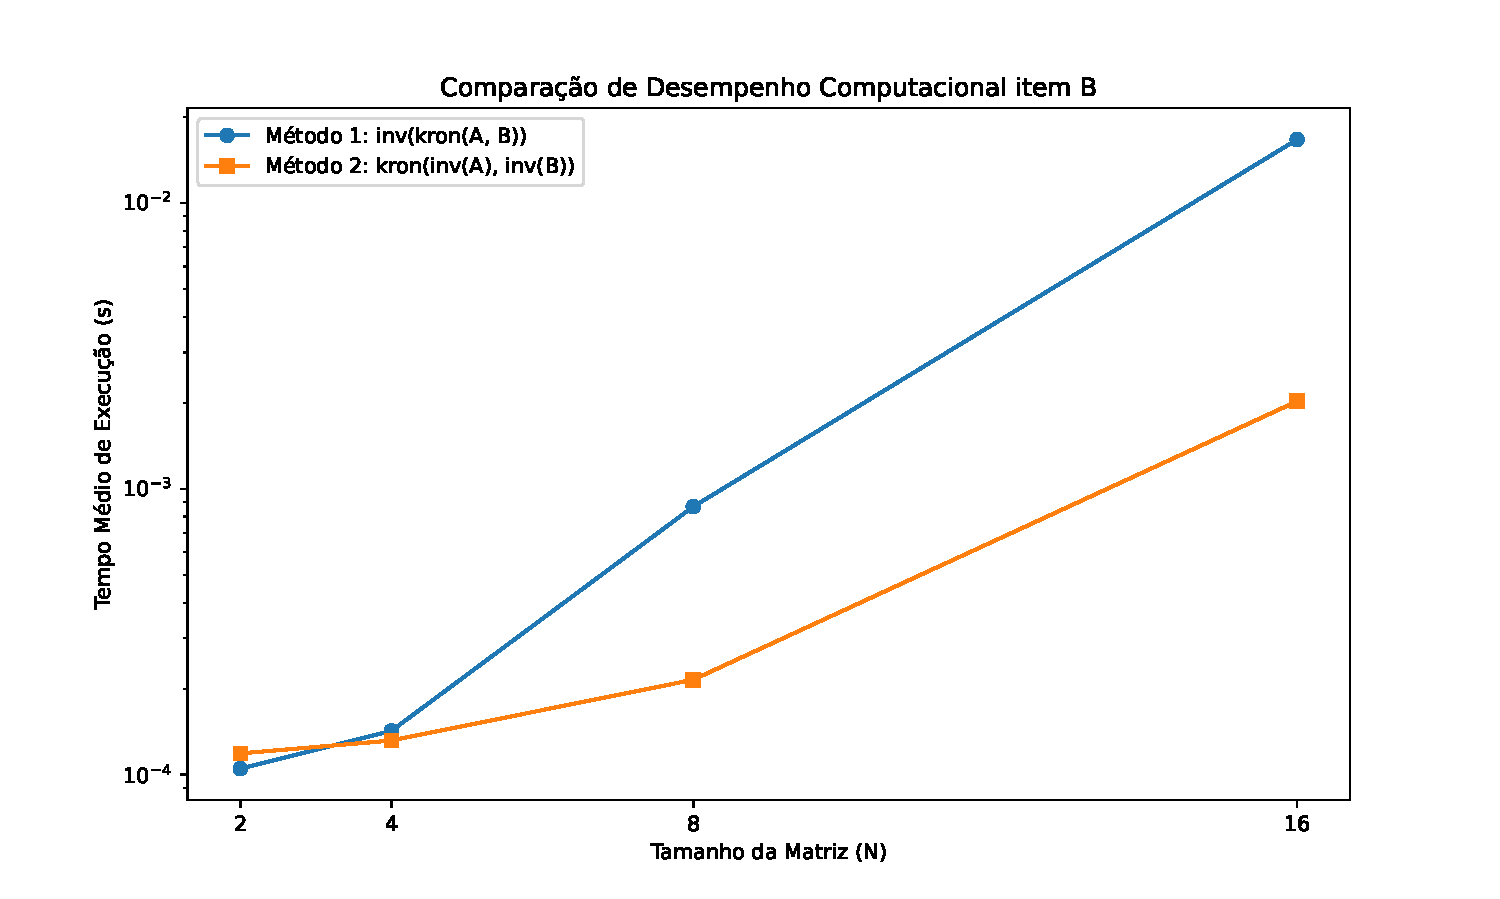
\includegraphics[width=0.9\linewidth]{itema.pdf}
		\caption{Tempo de compilação de acordo com N para cada um dos métodos}
		\label{fig:placeholder}
	\end{figure}
	
	Para o item b: 
	
	\begin{figure}[!h]
		\centering
		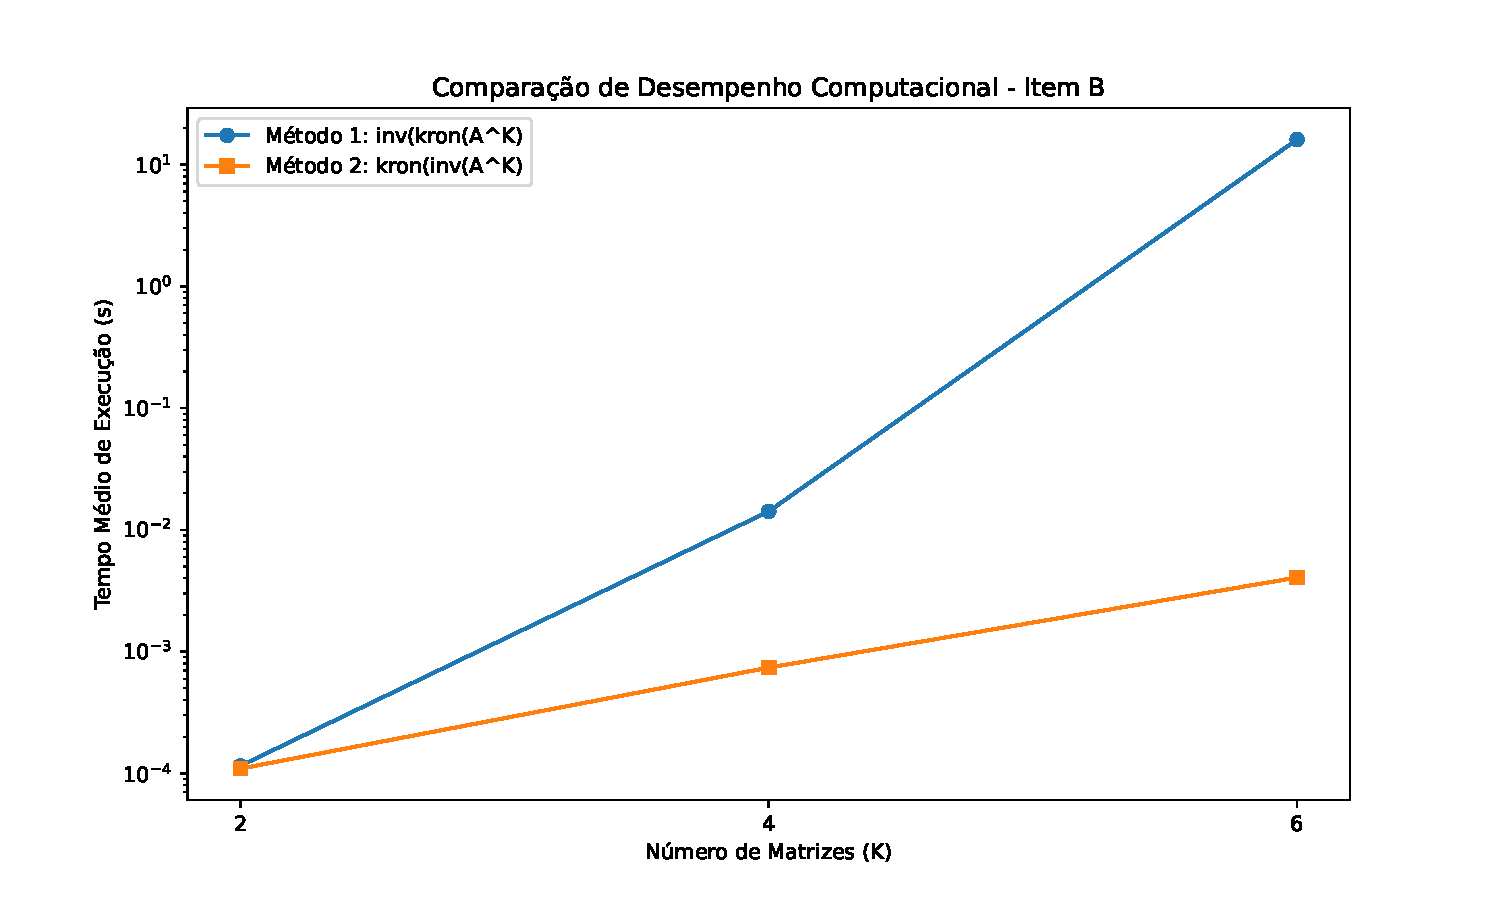
\includegraphics[width=0.9\linewidth]{itemb.pdf}
		\caption{Tempo de compilação de acordo com K para um dos métodos}
		\label{fig:placeholder}
	\end{figure}
	
	\newpage
	
	O código utilizado para montar as figuras segue abaixo:
	
	\begin{lstlisting}
		import time
		import numpy as np
		import matplotlib.pyplot as plt
		from tqdm import tqdm
		
		# para o item a do primeiro problema
		N = [2,4,8,16]  
		# 32 e 64 nao foram testados devido ao tempo de execucao
		
		time_met1 = np.zeros(len(N))
		time_met2 = np.zeros(len(N))
		
		inter_max = 1000
		for nn in range(len(N)):
		for i in tqdm(range(len(N))):
		time.sleep(0.01)
		current_n = N[nn]
		for i in range(inter_max):
		A = np.random.randn(current_n, current_n) 
		+ 1j * np.random.randn(current_n, current_n)
		B = np.random.randn(current_n, current_n) 
		+ 1j * np.random.randn(current_n, current_n)
		# para o metodo 1
		start_time = time.time()
		kron_prod = np.kron(A, B)
		np.linalg.inv(kron_prod)
		end_time = time.time()
		time_met1[nn] += end_time - start_time
		print(f"tempo do metodo 1: {time_met1[nn]}")
		# para o metodo 2
		start_time = time.time()
		inv_A = np.linalg.inv(A)
		inv_B = np.linalg.inv(B)
		np.kron(inv_A, inv_B)
		end_time = time.time()
		time_met2[nn] += end_time - start_time
		print(f"tempo do metodo 2: {time_met2[nn]}")
		
		# calculando o tempo medio
		time_met1 /= inter_max
		time_met2 /= inter_max
		
		print(f"tempo medio do metodo 1: {time_met1}")
		print(f"tempo medio do metodo 2: {time_met2}")
		
		plt.figure(figsize=(10, 6))
		plt.plot(N, time_met1, 'o-', label='Metodo 1: inv(kron(A, B))')
		plt.plot(N, time_met2, 's-', 
		label='Metodo 2: kron(inv(A), inv(B))')
		plt.xlabel("Tamanho da Matriz (N)")
		plt.ylabel("Tempo Medio de Execucao (s)")
		plt.title("Comparacao de Desempenho Computacional item A")
		plt.legend()
		plt.yscale('log')
		plt.xticks(N)
		plt.show()
		
		# para o item b do primeiro problema
		K = [2, 4, 6] 
		# 8 e 10 nao foram testados devido ao tempo de execucao
		N = 4
		
		timeb_met1 = np.zeros(len(K))
		timeb_met2 = np.zeros(len(K))
		
		inter_max = 1000
		for kk in range(len(K)):
		for i in tqdm(range(len(K))):
		time.sleep(0.01)
		current_k = K[kk]
		for i in range(inter_max):
		A = [np.random.randn(N,N) 
		+ 1j * np.random.randn(N,N)
		for _ in range(current_k)]
		# para o metodo 1
		start_time = time.time()
		kron_prod = A[0]
		if current_k > 1:
		for i in range(1, current_k):
		kron_prod = np.kron(kron_prod, A[i])
		np.linalg.inv(kron_prod)
		end_time = time.time()
		timeb_met1[kk] += end_time - start_time
		#print(f"tempo do metodo 1: {timeb_met1[kk]}")
		# para o metodo 2
		start_time = time.time()
		inv_A = [np.linalg.inv(A[i]) 
		for _ in range(current_k)]
		kron_prod_inv = inv_A[0]
		if current_k > 1:
		for i in range(1, current_k):
		kron_prod = 
		np.kron(kron_prod_inv, inv_A[i])
		end_time = time.time()
		timeb_met2[kk] += end_time - start_time
		#print(f"tempo do metodo 2: {timeb_met2[kk]}")
		
		# Calcula o tempo medio
		timeb_met1 /= inter_max
		timeb_met2 /= inter_max
		
		print(f"tempo medio do metodo 1 item b: {timeb_met1}")
		print(f"tempo medio do metodo 2 item b: {timeb_met2}")
		
		plt.figure(figsize=(10,6))
		plt.plot(K, timeb_met1, 'o-', label='Metodo 1: inv(kron(A^K)')
		plt.plot(K, timeb_met2, 's-', label='Metodo 2: kron(inv(A^K)')
		plt.xlabel("Numero de Matrizes (K)")
		plt.ylabel("Tempo Medio de Execucao (s)")
		plt.title("Comparacao de Desempenho Computacional - Item B")
		plt.legend()
		plt.yscale('log')
		plt.xticks(K)
		plt.show()
	\end{lstlisting}
	
	Para o segundo problema, precisamos encontrar uma forma de mostrar que, se $\lambda$ é $eig(A)$ e $\mu$ é $eig(B)$, então o produto $\lambda\mu$ deve ser equivalente a $eig(A \otimes B)$.
	
	Considerando que $\lambda$ seja um autovalor de A, ele terá um autovetor, que chamaremos de $v$. Assim, teremos que: 
	
	\begin{equation}
		A\mathbf{v} = \lambda \mathbf{v}    
	\end{equation}
	
	Da mesma forma, para B, seja $\mu$ um autovalor de $B$, com $\mathbf{w}$ sendo seu autovetor. Temos:
	
	
	\begin{equation}
		B\mathbf{w} = \mu \mathbf{w}
	\end{equation}
	
	
	Supomos então que o autovetor para $A \otimes B$ seja o produto de Kronecker dos autovetores individuais, ou seja, o vetor $\mathbf{v} \otimes \mathbf{w}$.
	
	Multiplicando ambos, temos: 
	
	
	\begin{equation}
		(A \otimes B)(\mathbf{v} \otimes \mathbf{w})
	\end{equation}
	
	Dai, pelo produto misto:
	
	\begin{equation}
		(A \otimes B)(\mathbf{v} \otimes \mathbf{w}) = (A\mathbf{v}) \otimes (B\mathbf{w})
	\end{equation}
	
	Substituindo a partir da relação encontrada em (1) e (2) no lado direito:
	
	\begin{equation}
		(\lambda \mathbf{v}) \otimes (\mu \mathbf{w})
	\end{equation}
	
	Podemos então retirar os escalares de dentro do produto de Kronecker por propriedade:
	
	\begin{equation}
		\lambda\mu (\mathbf{v} \otimes \mathbf{w})
	\end{equation}
	
	Por fim, temos: 
	
	\begin{equation}
		(A \otimes B)(\mathbf{v} \otimes \mathbf{w}) = (\lambda\mu)(\mathbf{v} \otimes \mathbf{w})
	\end{equation}
	
	o que satisfaz as condições. 
	
	\section{Homework 01}
	
	Para o problema 1, foi feito primeiro uma multiplicação utilizando uma função de uma biblioteca, e depois executando uma multiplicação por cada elemento, tal qual a operação de Hadamard.
	
	Da mesma forma, foi realizado as outras operações. 
	
	Assim, temos: 
	
	\begin{figure}[h!]
		\centering
		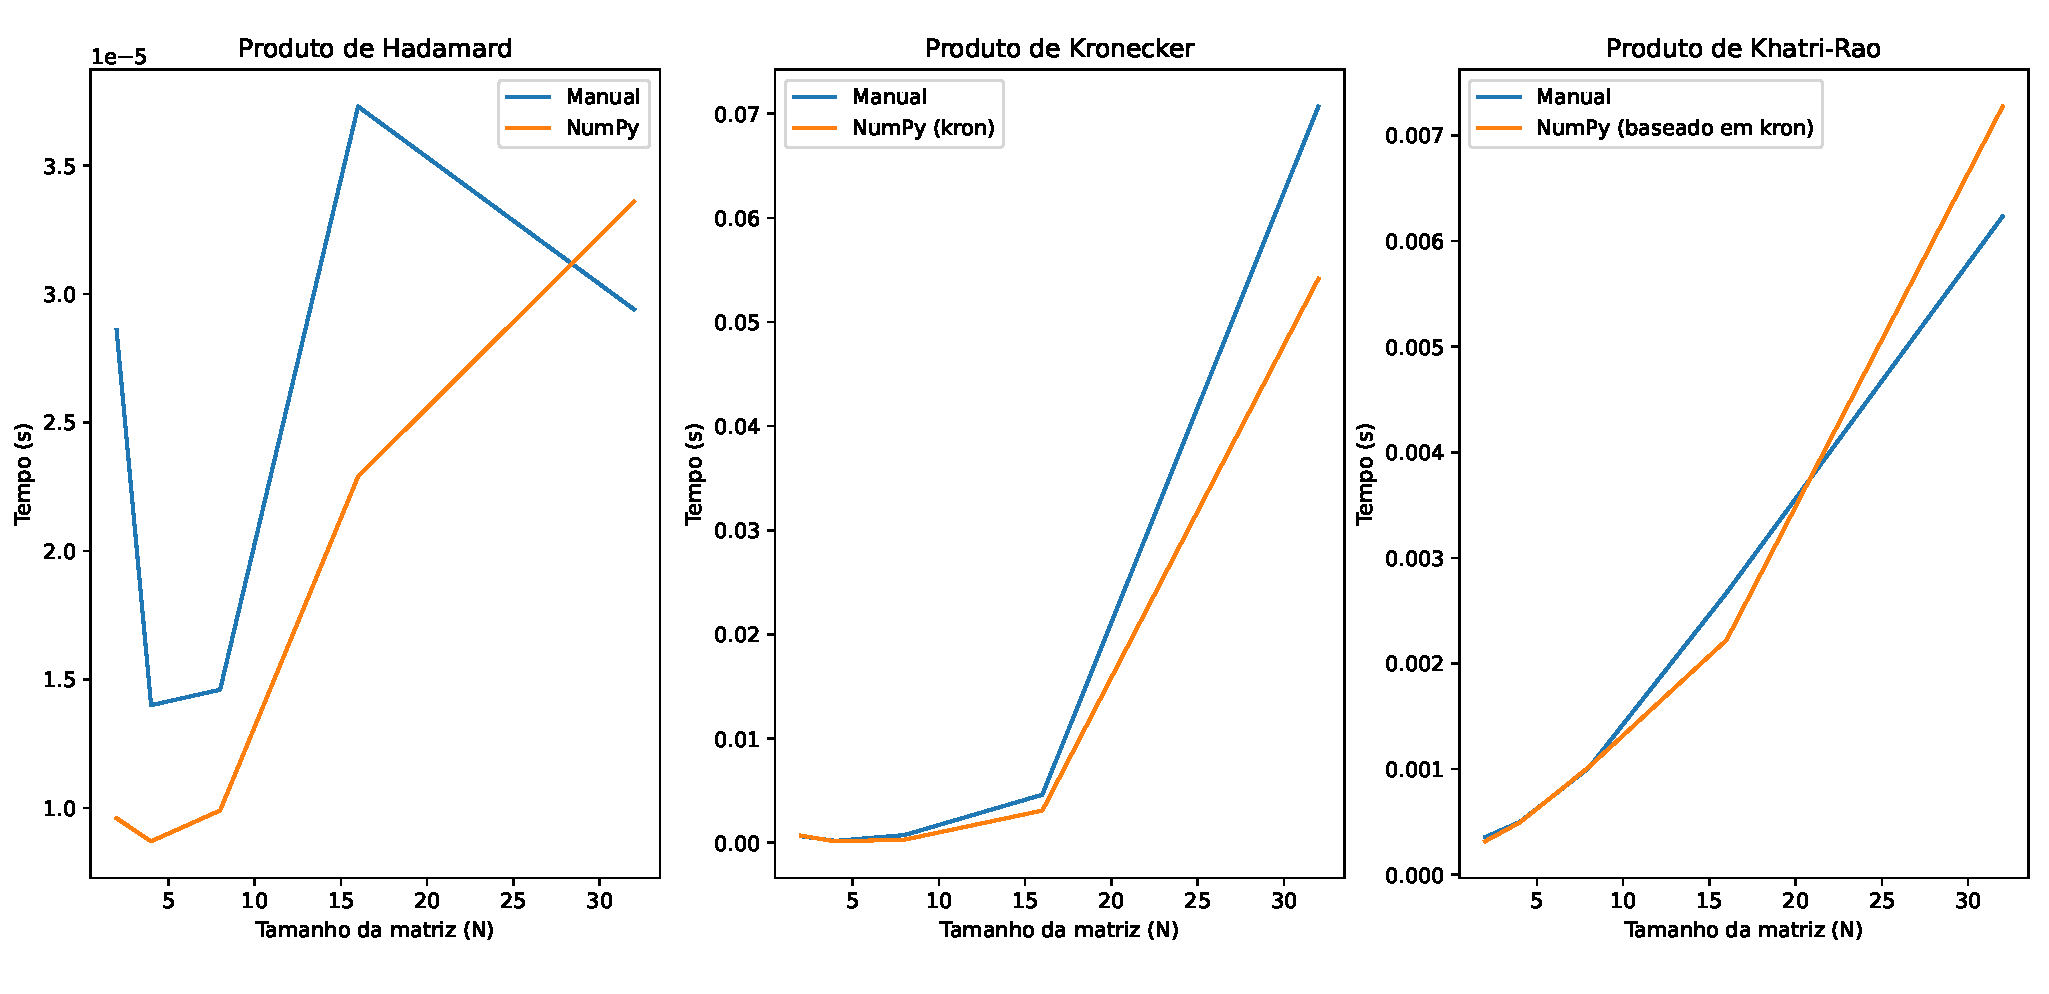
\includegraphics[width=0.9\linewidth]{images/comparativo_operacoes.pdf}
		\caption{Multiplicação manual vs operador multiplicador}
		\label{fig:comparativo}
	\end{figure}
	
	cuja Figura \ref{fig:comparativo} foi feita a partir do seguinte código:
	
	\begin{lstlisting}
		import numpy as np
		import timeit
		import matplotlib.pyplot as plt
		
		# Problema 1: Produto de Hadamard
		def hadamard_product(A, B):
		"""Implementacao manual do produto de Hadamard"""
		if A.shape != B.shape:
		raise ValueError("Matrizes devem ter as 
		mesmas dimensoes para o produto de Hadamard")
		return np.multiply(A, B)  # Na pratica, seria: 
		A * B (element-wise)
		
		# Problema 2: Produto de Kronecker
		def kronecker_product(A, B):
		"""Implementacao manual do produto de Kronecker"""
		m, n = A.shape
		p, q = B.shape
		result = np.zeros((m*p, n*q), dtype=A.dtype)
		
		for i in range(m):
		for j in range(n):
		result[i*p:(i+1)*p, j*q:(j+1)*q] = A[i,j] * B
		return result
		
		# Problema 3: Produto de Khatri-Rao
		def kr(A, B):
		"""Implementacao do produto de Khatri-Rao"""
		m, n = A.shape
		p, q = B.shape
		
		if n != q:
		raise ValueError("Para o produto Khatri-Rao, o numero de colunas deve ser igual")
		
		result = np.zeros((m*p, n), dtype=A.dtype)
		
		for j in range(n):
		# Produto de Kronecker das colunas j de A e B
		result[:, j] = np.kron(A[:, j], B[:, j])
		
		return result
		
		# Funcao para medir tempos de execucao
		def benchmark():
		sizes = [2, 4, 8, 16, 32] 
		#64 e 128 removidos por conta do tempo de compilacao
		hadamard_times_manual = []
		hadamard_times_np = []
		kronecker_times_manual = []
		kronecker_times_np = []
		khatri_rao_times_manual = []
		khatri_rao_times_np = []
		
		for N in sizes:
		A = np.random.rand(N, N) + 1j * np.random.rand(N, N)
		B = np.random.rand(N, N) + 1j * np.random.rand(N, N)
		
		# Benchmark Hadamard
		t = timeit.timeit(lambda: 
		hadamard_product(A, B), number=10)
		hadamard_times_manual.append(t)
		
		t = timeit.timeit(lambda: A * B, number=10)
		hadamard_times_np.append(t)
		
		# Benchmark Kronecker
		t = timeit.timeit(lambda: 
		kronecker_product(A, B), number=5)
		kronecker_times_manual.append(t)
		
		t = timeit.timeit(lambda: np.kron(A, B), number=5)
		kronecker_times_np.append(t)
		
		# Benchmark Khatri-Rao (assumindo N colunas)
		t = timeit.timeit(lambda: kr(A, B), number=5)
		khatri_rao_times_manual.append(t)
		
		# Nao ha funcao direta no NumPy para Khatri-Rao,
		usaremos uma implementacao baseada em Kronecker
		t = timeit.timeit(lambda: 
		np.concatenate([np.kron(A[:,j:j+1], B[:,j:j+1])
		for j in range(N)], axis=1), number=5)
		khatri_rao_times_np.append(t)
		
		# Plotar resultados
		plt.figure(figsize=(15, 5))
		
		# Hadamard
		plt.subplot(1, 3, 1)
		plt.plot(sizes, hadamard_times_manual, label='Manual')
		plt.plot(sizes, hadamard_times_np, label='NumPy')
		plt.title('Produto de Hadamard')
		plt.xlabel('Tamanho da matriz (N)')
		plt.ylabel('Tempo (s)')
		plt.legend()
		
		# Kronecker
		plt.subplot(1, 3, 2)
		plt.plot(sizes, kronecker_times_manual, label='Manual')
		plt.plot(sizes, kronecker_times_np, 
		label='NumPy (kron)')
		plt.title('Produto de Kronecker')
		plt.xlabel('Tamanho da matriz (N)')
		plt.ylabel('Tempo (s)')
		plt.legend()
		
		# Khatri-Rao
		plt.subplot(1, 3, 3)
		plt.plot(sizes, khatri_rao_times_manual, label='Manual')
		plt.plot(sizes, khatri_rao_times_np, 
		label='NumPy (baseado em kron)')
		plt.title('Produto de Khatri-Rao')
		plt.xlabel('Tamanho da matriz (N)')
		plt.ylabel('Tempo (s)')
		plt.legend()
		
		plt.tight_layout()
		plt.show()
		
		# Executar benchmark
		if __name__ == "__main__":
		benchmark()
	\end{lstlisting}
	
	Para o problema 2, similarmente, 
	
	\section{Homework 02}
	
	Para o primeiro problema, foi implementado cada uma das operações e feito a comparação temporal, de acordo com os valores de linhas e colunas, por meio de Monte Carlo. Da mesma forma, o número de I foi limitado devido a restrições computacionais. 
	
	Obtemos então como resultados:
	
	\begin{figure}[!h]
		\centering
		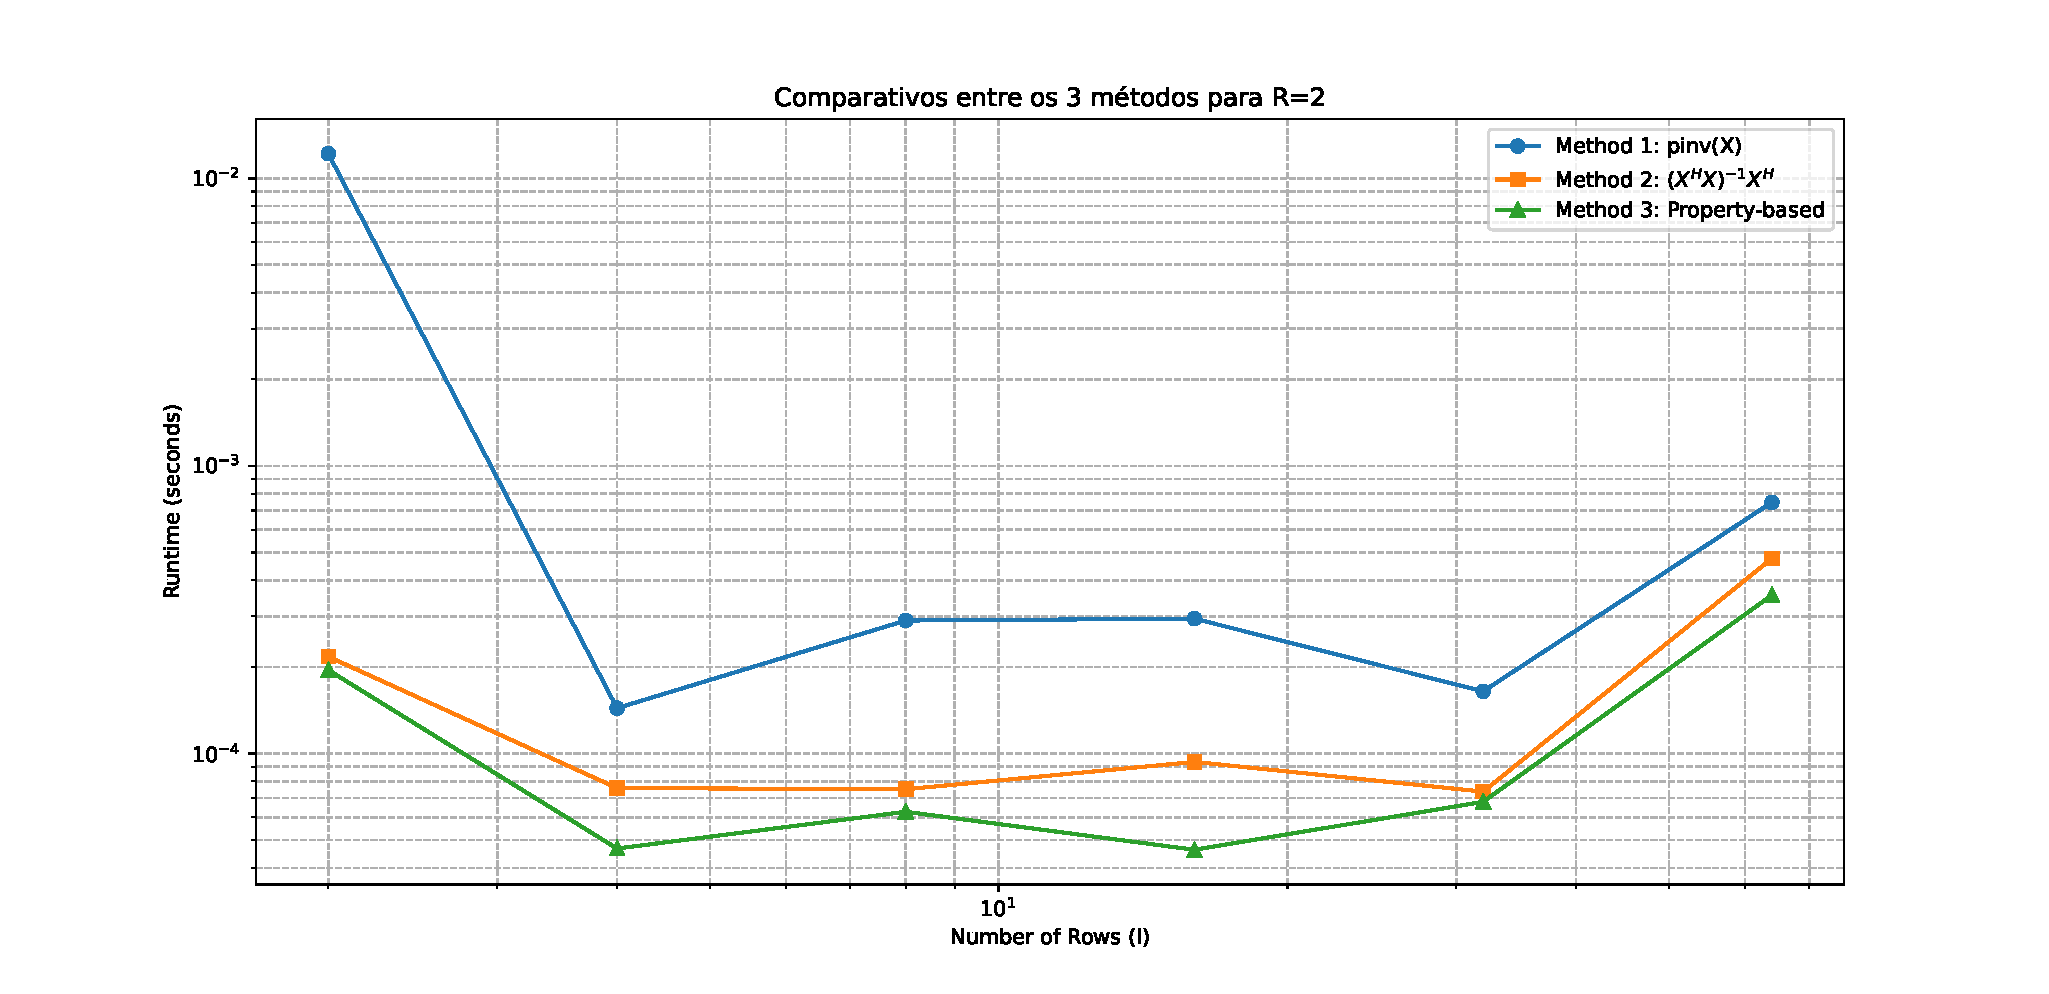
\includegraphics[width=\linewidth]{images/3met_r2.pdf}
		\caption{Comparativo dos 3 métodos para R = 2 de acordo com I}
		\label{fig:3metr2}
	\end{figure}
	
	\begin{figure}
		\centering
		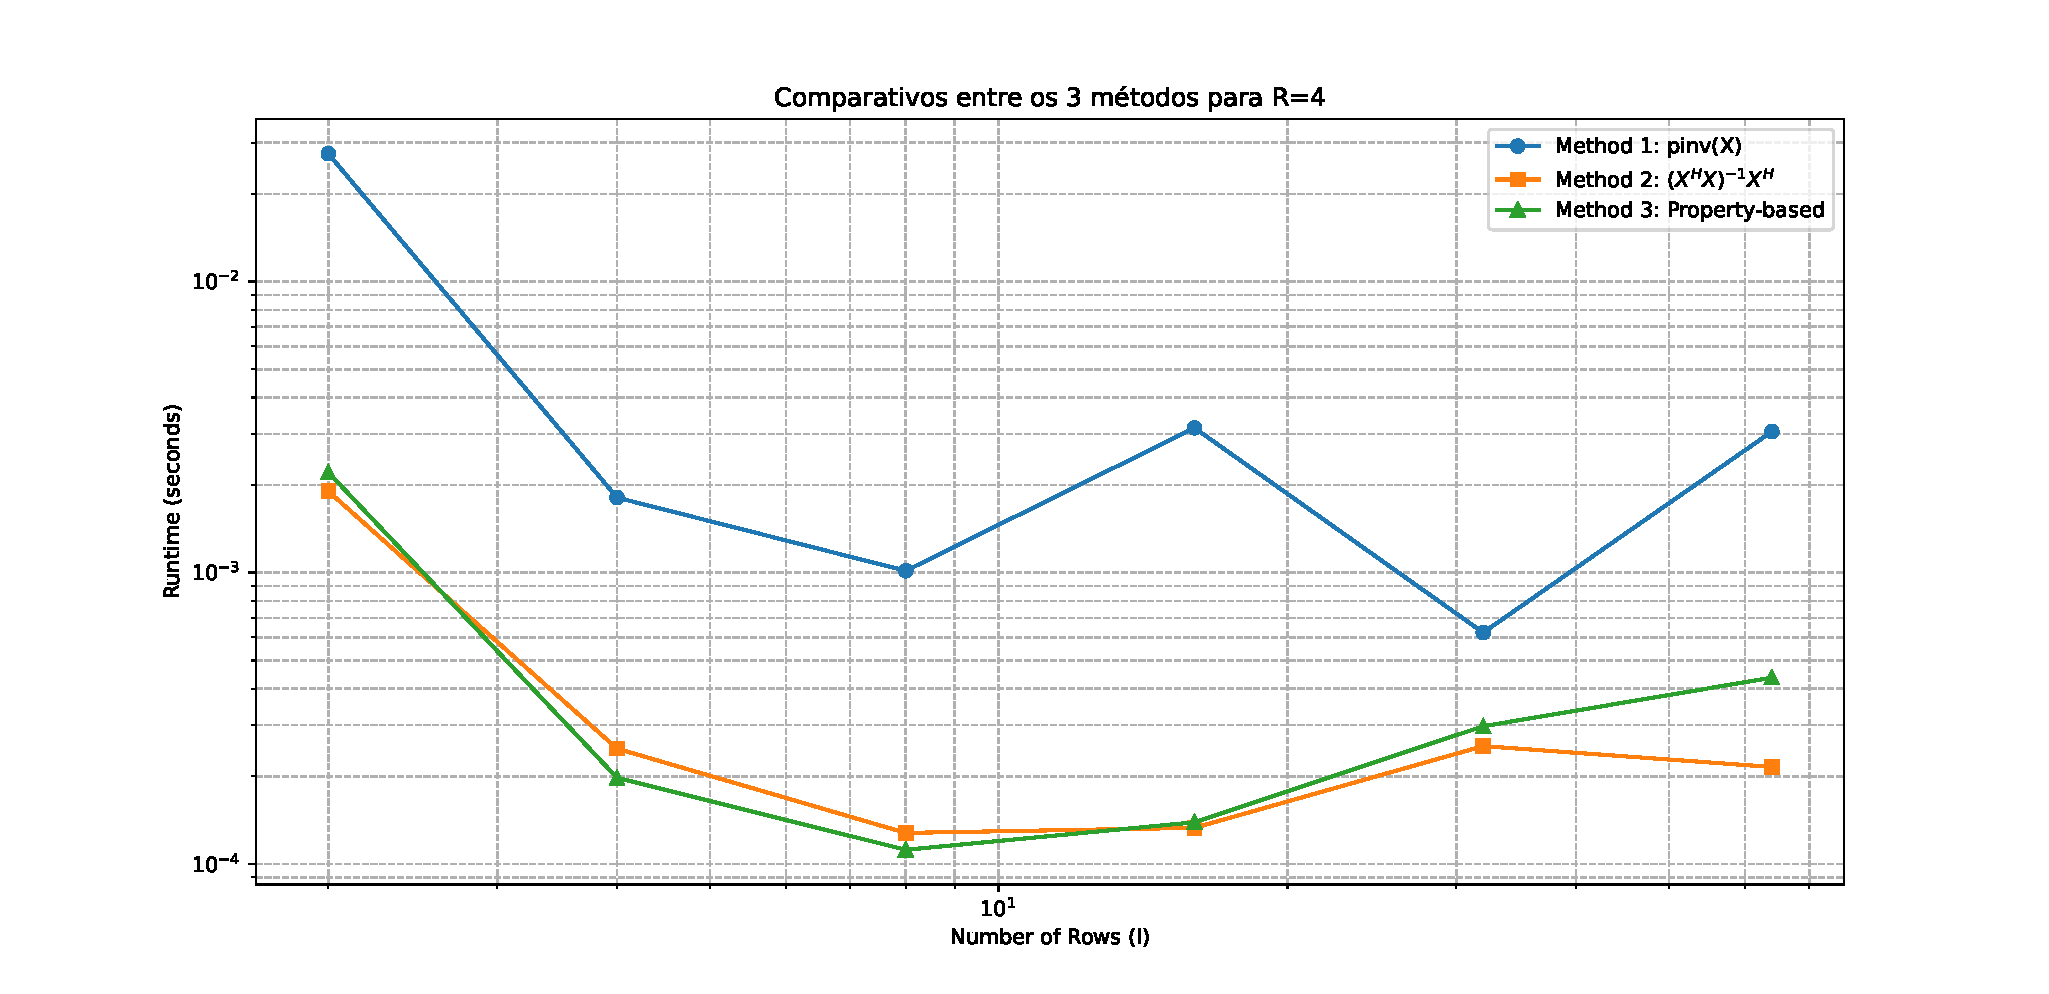
\includegraphics[width=\linewidth]{images/3met_r4.pdf}
		\caption{Comparativo dos 3 métodos para R = 4 de acordo com I}
		\label{fig:3metr4}
	\end{figure}
	
	O código utilizado foi o que segue:
	
	\begin{lstlisting}
		import numpy as np
		import time
		import matplotlib.pyplot as plt
		
		def khatri_rao(A, B):
		if A.shape[1] != B.shape[1]:
		raise ValueError("Matrizes devem ter o mesmo 
		numero de colunas.")
		
		C = np.zeros((A.shape[0] * B.shape[0], A.shape[1]))
		for i in range(A.shape[1]):
		C[:, i] = np.kron(A[:, i], B[:, i])
		return C
		
		I_values = [2, 4, 8, 16, 32, 64] 
		# 128, 256 foram retirados devido ao tempo de execucao
		R = 4
		
		times1 = []
		times2 = []
		times3 = []
		
		for I in I_values:
		print(f"Testing for I = {I}, R = {R}")
		
		A = np.random.randn(I, R) + 1j * np.random.randn(I, R)
		B = np.random.randn(I, R)
		
		X = khatri_rao(A, B)
		
		#metodo 1: pinv
		start_time = time.time()
		pinv_X1 = np.linalg.pinv(X)
		end_time = time.time()
		times1.append(end_time - start_time)
		
		# metodo 2: (X^H * X)^-1 * X^H
		start_time = time.time()
		X_H = X.conj().T
		XHX = X_H @ X
		XHX_inv = np.linalg.inv(XHX)
		pinv_X2 = XHX_inv @ X_H
		end_time = time.time()
		times2.append(end_time - start_time)
		
		# metodo 3: (A^H A) * (B^H B)
		start_time = time.time()
		A_H = A.conj().T
		B_T = B.T
		AHA = A_H @ A
		BTB = B_T @ B
		XHX_prop = AHA * BTB
		XHX_prop_inv = np.linalg.inv(XHX_prop)
		pinv_X3 = XHX_prop_inv @ X_H # usando X_H do metodo 2
		end_time = time.time()
		times3.append(end_time - start_time)
		
		# plot
		plt.figure(figsize=(12, 8))
		plt.loglog(I_values, times1, 'o-', label='Method 1: pinv(X)')
		plt.loglog(I_values, times2, 's-', 
		label=r'Method 2: $(X^H X)^{-1} X^H$')
		plt.loglog(I_values, times3, '^-', 
		label='Method 3: Property-based')
		plt.title('Comparativos entre os 3 metodos para R=4')
		plt.xlabel('Number of Rows (I)')
		plt.ylabel('Runtime (seconds)')
		plt.legend()
		plt.grid(True, which="both", ls="--")
		plt.show()
	\end{lstlisting}
	
	Para o problema 2, foi tirada a média do tempo total das operações de acordo com o número total de iterações. 
	
	Dessa forma, segue o resultado:
	\begin{figure}[!h]
		\centering
		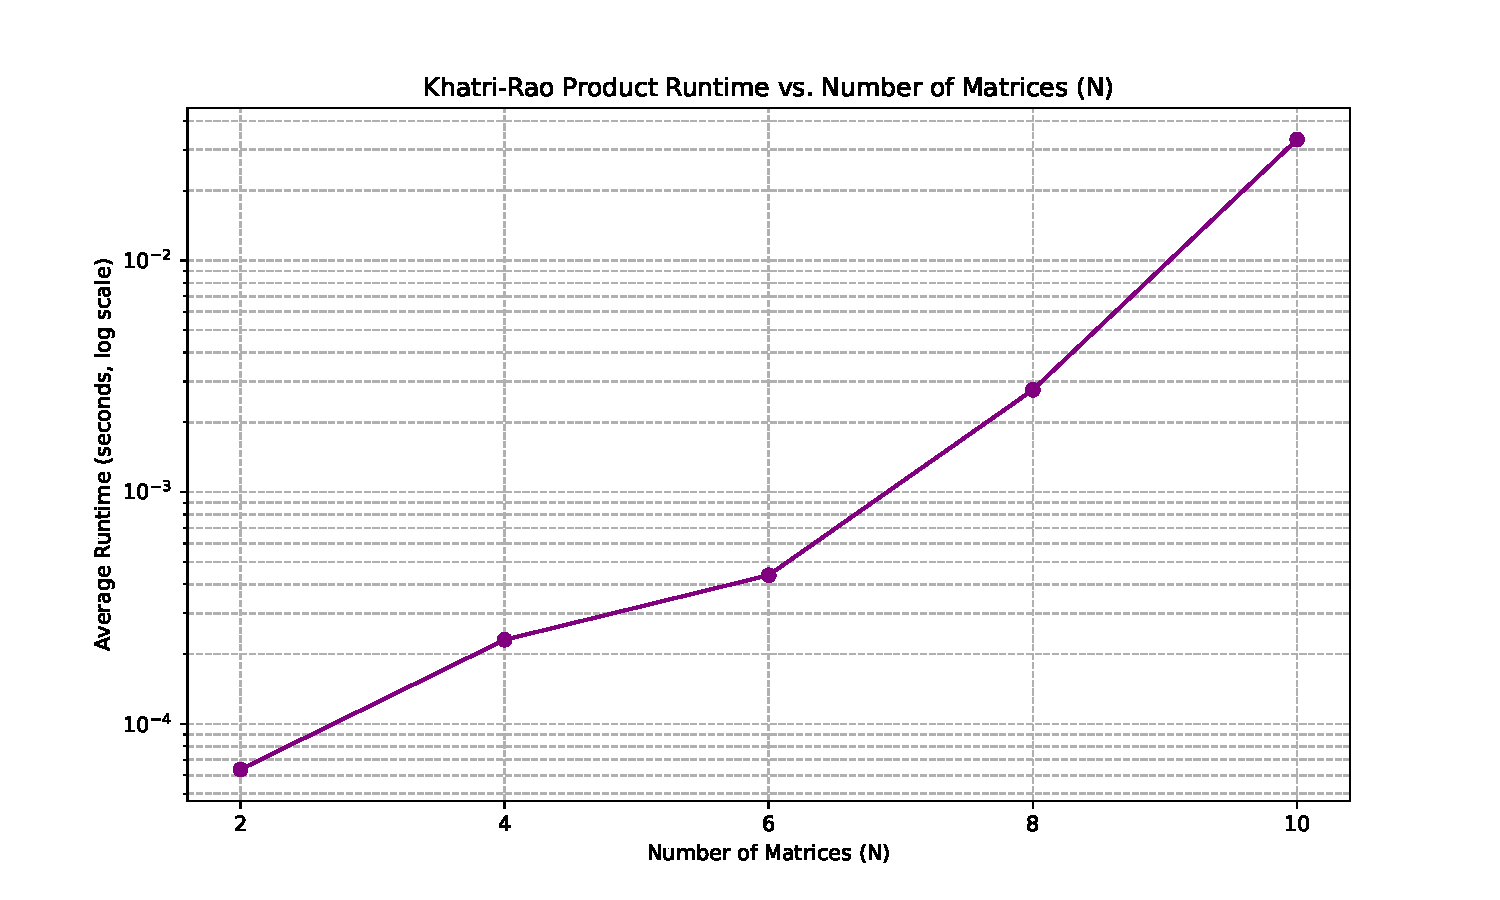
\includegraphics[width=\linewidth]{images/chained.pdf}
		\caption{Comparativo de tempo de operações em sequência de acordo com 50 iterações, para N matrizes}
		\label{fig:chained}
	\end{figure}
	
	O código segue:
	\begin{lstlisting}
		import numpy as np
		import time
		import matplotlib.pyplot as plt
		
		def khatri_rao(A, B):
		if A.shape[1] != B.shape[1]:
		raise ValueError("Matrizes devem ter o mesmo número de colunas.")
		
		C = np.zeros((A.shape[0] * B.shape[0], A.shape[1]))
		for i in range(A.shape[1]):
		C[:, i] = np.kron(A[:, i], B[:, i])
		return C
		
		# para o problema 1
		I_values = [2, 4, 8, 16, 32, 64] # 128, 256 foram retirados devido ao tempo de execução
		R = 4
		
		times1 = []
		times2 = []
		times3 = []
		
		for I in I_values:
		print(f"Testing for I = {I}, R = {R}")
		
		A = np.random.randn(I, R) + 1j * np.random.randn(I, R)
		B = np.random.randn(I, R)
		
		X = khatri_rao(A, B)
		
		#metodo 1: pinv
		start_time = time.time()
		pinv_X1 = np.linalg.pinv(X)
		end_time = time.time()
		times1.append(end_time - start_time)
		
		# metodo 2: (X^H * X)^-1 * X^H
		start_time = time.time()
		X_H = X.conj().T
		XHX = X_H @ X
		XHX_inv = np.linalg.inv(XHX)
		pinv_X2 = XHX_inv @ X_H
		end_time = time.time()
		times2.append(end_time - start_time)
		
		# metodo 3: (A^H A) * (B^H B)
		start_time = time.time()
		A_H = A.conj().T
		B_T = B.T
		AHA = A_H @ A
		BTB = B_T @ B
		XHX_prop = AHA * BTB
		XHX_prop_inv = np.linalg.inv(XHX_prop)
		pinv_X3 = XHX_prop_inv @ X_H # usando X_H do metodo 2
		end_time = time.time()
		times3.append(end_time - start_time)
		
		# plot
		plt.figure(figsize=(12, 8))
		plt.loglog(I_values, times1, 'o-', label='Method 1: pinv(X)')
		plt.loglog(I_values, times2, 's-', label=r'Method 2: $(X^H X)^{-1} X^H$')
		plt.loglog(I_values, times3, '^-', label='Method 3: Property-based')
		plt.title('Comparativos entre os 3 métodos para R=4')
		plt.xlabel('Number of Rows (I)')
		plt.ylabel('Runtime (seconds)')
		plt.legend()
		plt.grid(True, which="both", ls="--")
		plt.show()
		
		# para o problema 2
		I = 4
		R = 2
		N = [2,4,6,8,10]
		max_inter = 50
		
		tempo = []
		
		for n in N:
		total_tempo = 0
		for _ in range(max_inter):
		# gerando as matrizes aleatorias
		A = [np.random.rand(I, R) for _ in range(n)]
		start_time = time.time()
		X = A[0]
		for m in range(1,n):
		X = khatri_rao(X, A[m])
		end_time = time.time()
		total_tempo += end_time - start_time
		tempo.append(total_tempo / max_inter)
		
		plt.figure(figsize=(10, 6))
		# A semi-log plot is best to visualize exponential growth
		plt.semilogy(N, tempo, 'o-', color='purple')
		
		plt.title('Khatri-Rao Product Runtime vs. Number of Matrices (N)')
		plt.xlabel('Number of Matrices (N)')
		plt.ylabel('Average Runtime (seconds, log scale)')
		plt.grid(True, which="both", ls="--")
		plt.xticks(N)
		plt.show()
		
		
	\end{lstlisting}
	
	\section{Homework 03}
	
	Para o problema 1, temos que simplesmente realizar a implementação do Least Square Katri Rao Factorization (LSKRF), seguindo de acordo com o enunciado.
	
	Segue o resultado: 
	
	
	% \section{Homework 09}
	
	% A ideia é decompor um tensor de ordem superior (neste caso, um tensor de terceira ordem $\mathcal{X}$) em uma soma de $R$ componentes de rank-1. Cada componente de rank-1 é o produto externo de $R$ vetores, ou seja o rank do tensor.
	
	% Onde $\mathbf{a}_r$, $\mathbf{b}_r$ e $\mathbf{c}_r$ são os $r$-ésimos vetores das matrizes fatoriais A, B e C, respectivamente, e $\circ$ denota o produto externo. Na prática, isso é equivalente a encontrar as matrizes fatoriais A, B e C.
	
\end{document}
